\section{DnsHeader}\label{sec:dnshdr}

\begin{figure}
\begin{center}
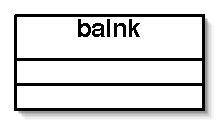
\includegraphics[width=0.4\textwidth]{figs/blank}
\end{center}
\caption{}
\label{fig:dnshdr}
\end{figure}

This section describes the DnsHeader component, which is described by Figure~\ref{fig:dnshdr}.  

This class holds the header information for a DNS packet, providing convenience methods for various data.

\subsection{Methods}

{\bf Public Methods}
\begin{itemize}
\item init(): Loads the header from a wire representation.
\item id(): Get the ID of the query.
\item qd\_count(): Get the query count.
\item an\_count(): Get the answer count.
\item ns\_count(): Get the authoritative NS count.
\item ar\_count(): Get the additional count.
\item response(): Is this a response?
\item rcode(): Get the RCODE.
\item to\_wire(): Convert to the wire format.
\end{itemize}

{\bf Private Methods}
\begin{itemize}
\item pack\_flags(): Pack flags into wire representation.
\item unpack\_flags(): Unpack flags into a common C-style structure.
\end{itemize}

\subsection{Member Variables}
\begin{itemize}
\item m\_init: True if packet has been initialized.
\item query\_id: Query ID of the packet.
\item flags: Header flags.
\item qdcount: Question count.
\item ancount: Answer count.
\item nscount: NS count.
\item arcount: Additional count.
\end{itemize}
